\documentclass[usenames,dvipsnames]{beamer}

\usetheme[bgphoto]{polimi}
% \usetheme{Madrid}
\usepackage[utf8]{inputenc}
\usepackage{appendixnumberbeamer}
\usepackage{array,multirow,booktabs}
\usepackage{lipsum}
\usepackage[font=scriptsize]{caption}
\usepackage{subfig}

% Full instructions available at:
% https://github.com/elauksap/beamerthemepolimi

\title{Gender Discrimination in Data Analysis:\\a Socio-Technical Approach}
\author{Riccardo Corona}
\date{07/10/2021}


\begin{document}
    \begin{frame}
        \maketitle
    \end{frame}
    
    
    \begin{frame}{Research Context}
        \begin{block}{Data analysis}
            Set of processes for inspecting, cleaning, transforming, and modeling data with the aim of discovering useful information, informing conclusions, and supporting decision making.
        \end{block}
        \begin{block}{Gender discrimination}
            Specific (sub)category of social problems, here expressed in the form of the so-called `\textbf{gender gap}', definable as:
            \begin{quote}
            \emph{A difference between the way men and women are treated in society, or between what men and women do and achieve.}
            \end{quote}
        \end{block}
    \end{frame}
    
    
    \begin{frame}{Scenarios \& Problem Statement}
        \begin{block}{Problem}
            Data and datasets, on which a lot of actions of our daily routine are based, can be \textbf {unfair}. Unfair, or better to say, \textbf{biased} data, may influence, directly or indirectly, our perception of reality, and lead us to make decisions that, although seemingly fair and just, contain in turn bias, and discriminate against individuals or groups of individuals.
        \end{block}
        \begin{exampleblock}{Example scenarios}
            \begin{itemize}
                \item \textcolor{greenPolimi}{COMPAS} tool used in the U.S. to predict recidivism risk biased against Black people (2016).
                \item \textcolor{greenPolimi}{Amazon} software to screen candidates for employment biased against women (2015).
            \end{itemize}
        \end{exampleblock}
    \end{frame}
    
    
    \begin{frame}{Sociological Perspective -- Data \& Statistics}
        \begin{figure}
            \subfloat{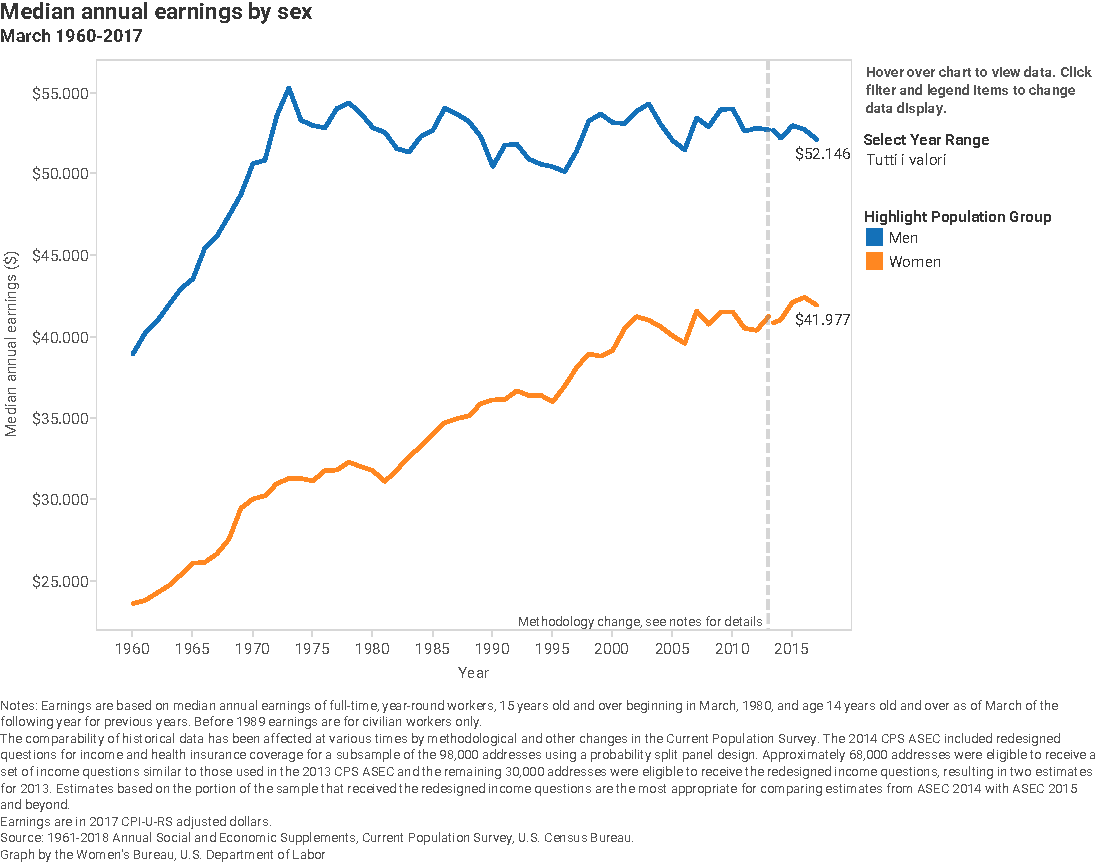
\includegraphics[width=0.475\textwidth]{figures/dol_earnings_by_sex.pdf}}
            \hfill
            \subfloat{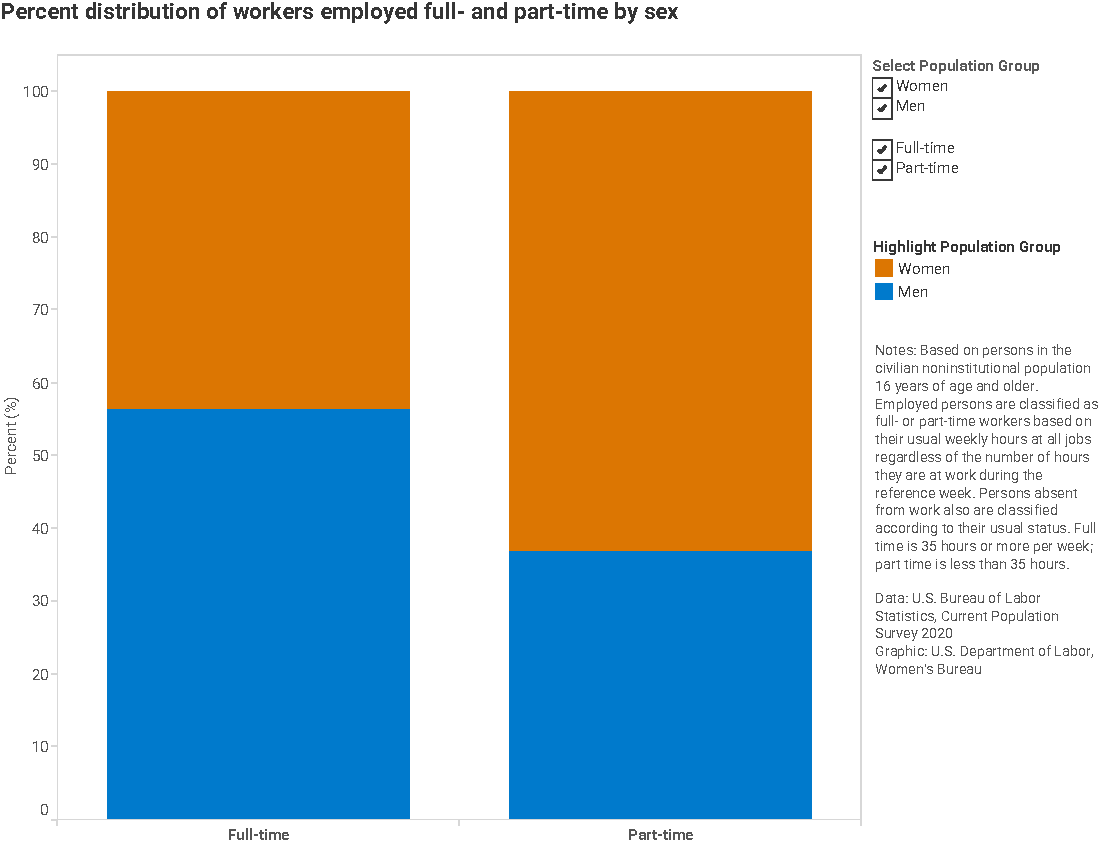
\includegraphics[width=0.475\textwidth]{figures/dol_full-_and_part-time_workers_by_sex.pdf}}
        \end{figure}
    \end{frame}
    
    
    \begin{frame}{Sociological Perspective -- Data \& Statistics}
        \begin{figure}
            \subfloat{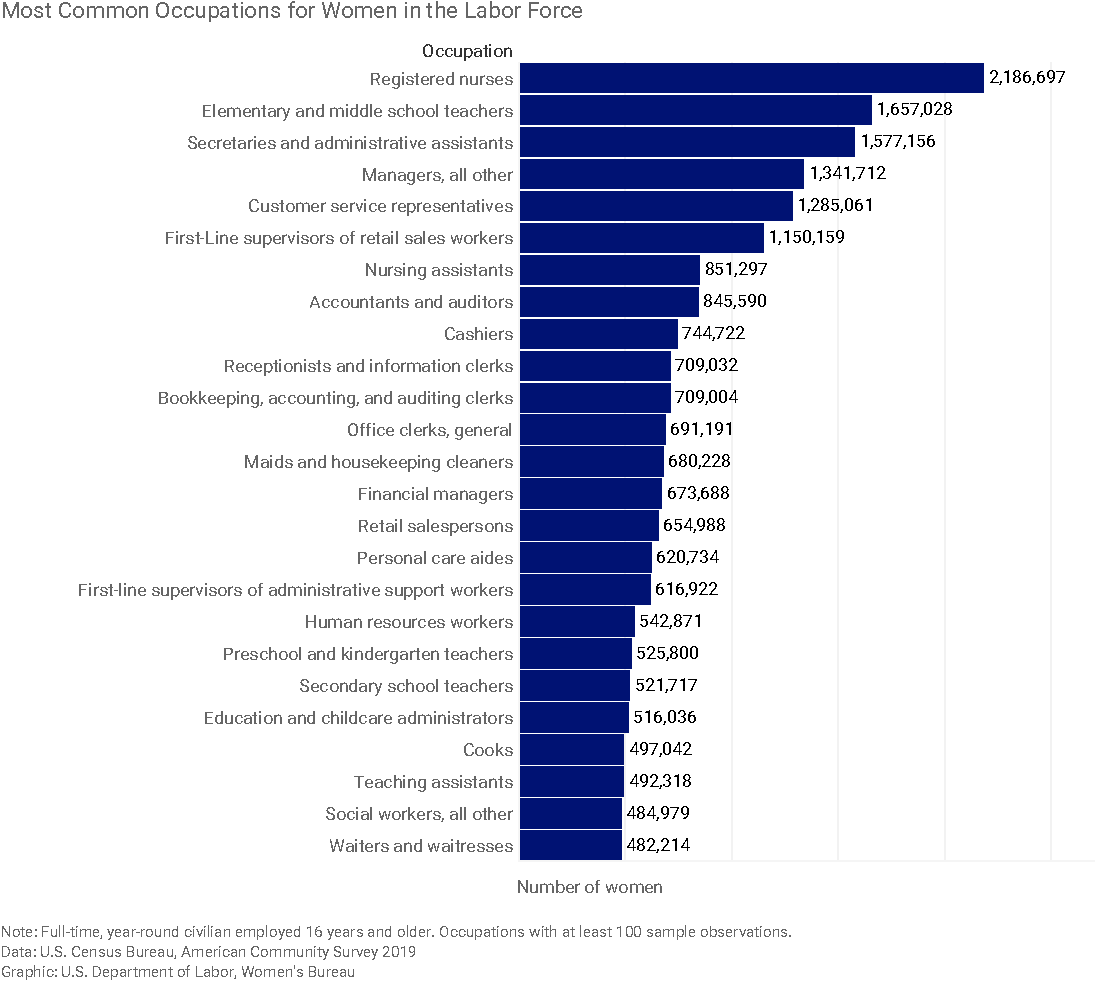
\includegraphics[width=0.475\textwidth]{figures/dol_most_common_occupations_women.pdf}}
            \hfill
            \subfloat{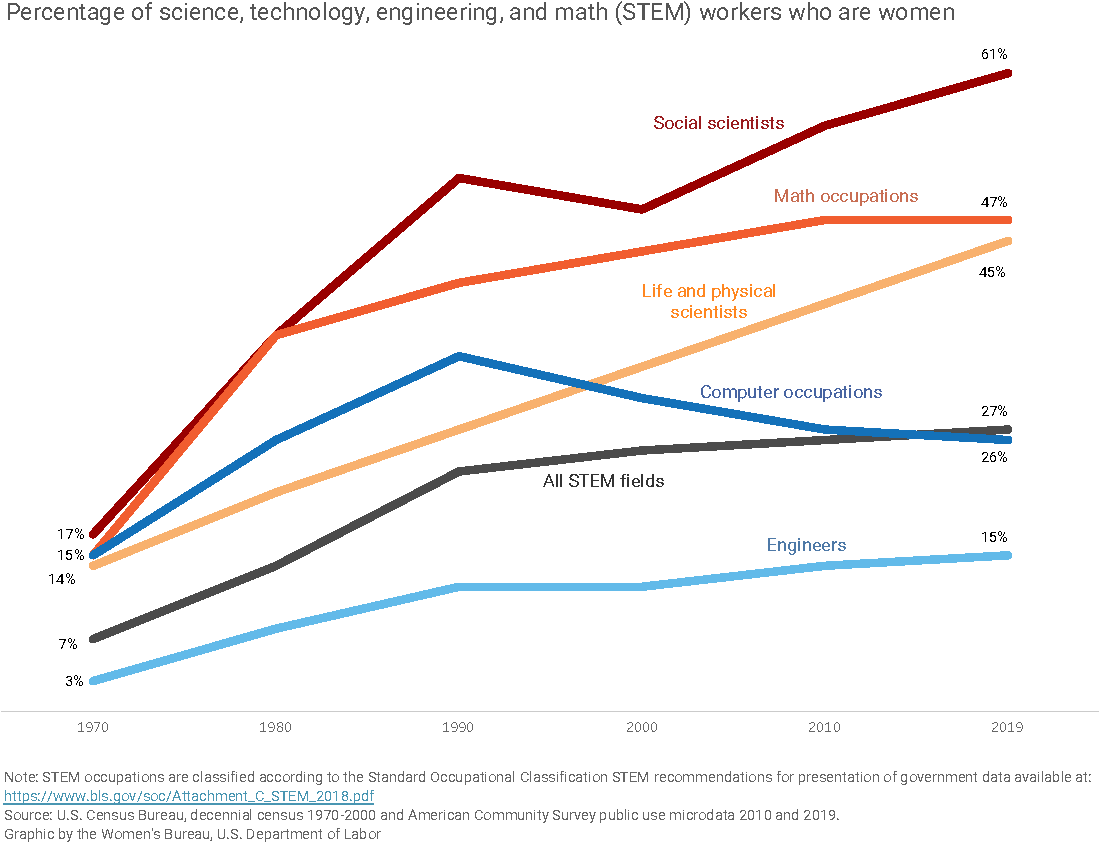
\includegraphics[width=0.475\textwidth]{figures/dol_stem_percent_women.pdf}}
        \end{figure}
    \end{frame}
    
    
    \begin{frame}{Tools for Assessing Fairness}
        \begin{itemize}
            \item \textit{The `Glassdoor Method'}: a framework for evaluating gender pay gap which relies on \textbf{linear regression}.
            \item \textit{FAIR-DB}: an algorithm to detect bias in data based on \textbf{functional dependencies} and the related evaluation metrics.
            \item \textit{Ranking Facts}: an application built on the idea of \textbf{ranking} which makes use of three statistical measures to evaluate fairness.
        \end{itemize}
    \end{frame}
    
    
    \begin{frame}{Case Study 1: Chicago}
        \begin{itemize}
            \item \textbf{Data Preprocessing}: 20,309 tuples, of which 16,146 males and 4,163 females, and with 35 distinct \textit{Job Title} values and 20 distinct \textit{Department} values.\newline
            \item \textbf{The `Glassdoor Method'}: 24.2\% `unadjusted' pay gap; 0.4\% `adjusted' pay gap $\rightarrow$ no evidence of a systematic gender pay gap.
            \item \textbf{FAIR-DB}: 6 final functional dependencies; 11.4\% of the dataset `problematic' $\rightarrow$ dataset quite fair.
            \item \textbf{Ranking Facts}: dataset fair for both males and females, for each statistical measure.
        \end{itemize}
    \end{frame}
    
    
    \begin{frame}{Case Study 1: Chicago}
        \begin{figure}
            \subfloat{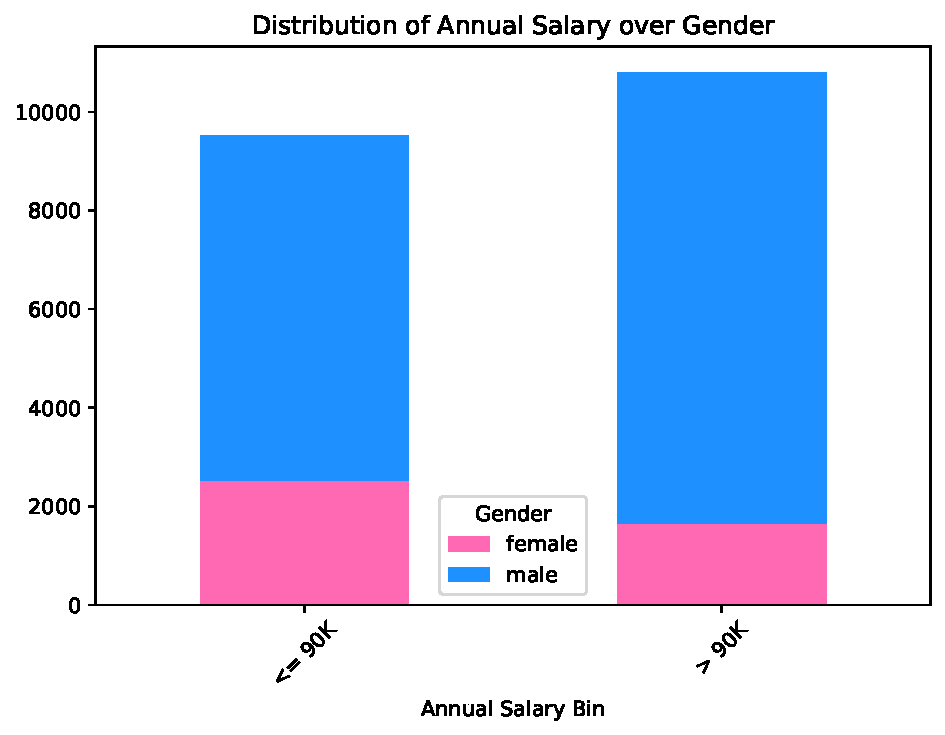
\includegraphics[width=0.475\textwidth]{figures/chicago_2bins_annual_salary_over_gender.pdf}}
            \hfill
            \subfloat{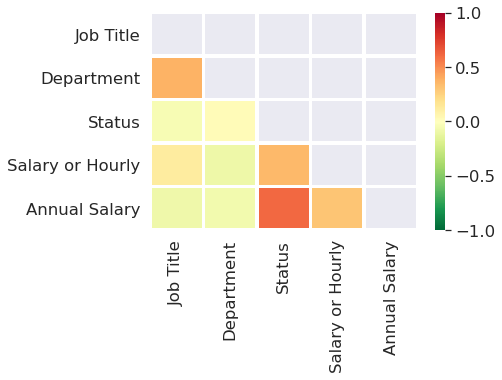
\includegraphics[width=0.475\textwidth]{figures/chicago_rankingfacts1.png}}
        \end{figure}
    \end{frame}
    
    
    \begin{frame}{Case Study 2: San Francisco}
        \begin{itemize}
            \item \textbf{Data Preprocessing}: 22,996 tuples, of which 13,688 males and 9,308 females, and with 81 distinct \textit{Job Title} values.\newline
            \item \textbf{The `Glassdoor Method'}: 30.4\% `unadjusted' pay gap; -0.5\% `adjusted' pay gap $\rightarrow$ no evidence of a systematic gender pay gap.
            \item \textbf{FAIR-DB}: 10 final functional dependencies; 24.3\% of the dataset `problematic' $\rightarrow$ dataset quite fair because of the low values of \textit{difference} (`unfairness level') and \textit{support} (number of tuples involved), but for higher-paying jobs men seem to have an economic advantage over women.
            \item \textbf{Ranking Facts}: dataset fair for males and unfair for females, for each statistical measure $\rightarrow$ proportion of women in the top-\(k\) ranking effectively very low.
        \end{itemize}
    \end{frame}
    
    
    \begin{frame}{Case Study 2: San Francisco}
        \begin{figure}
            \subfloat{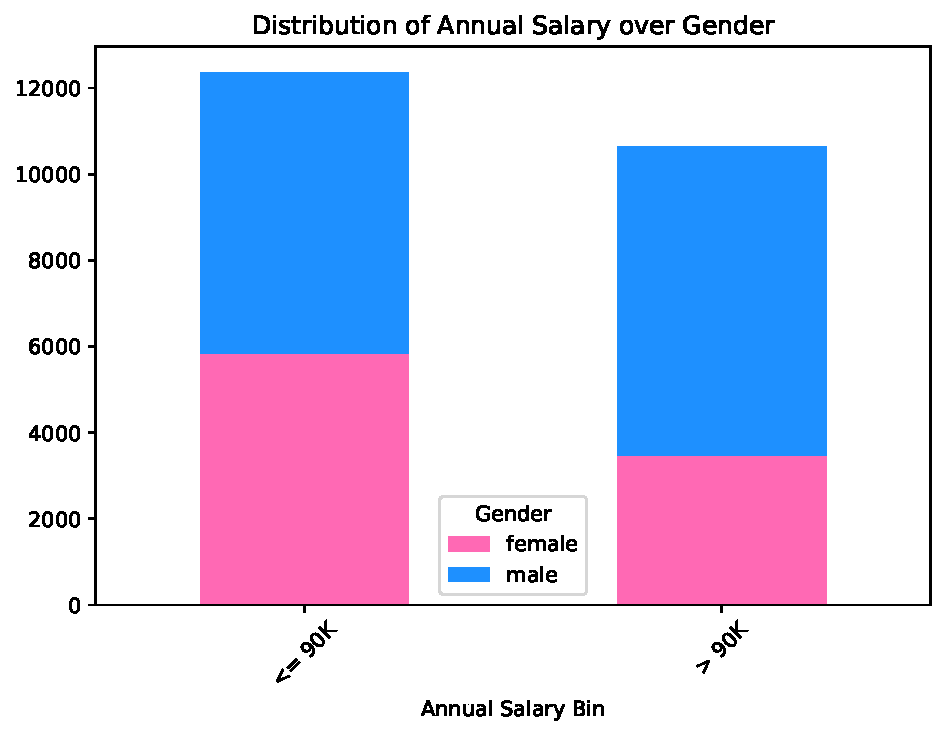
\includegraphics[width=0.475\textwidth]{figures/san_francisco_2bins_annual_salary_over_gender.pdf}}
            \hfill
            \subfloat{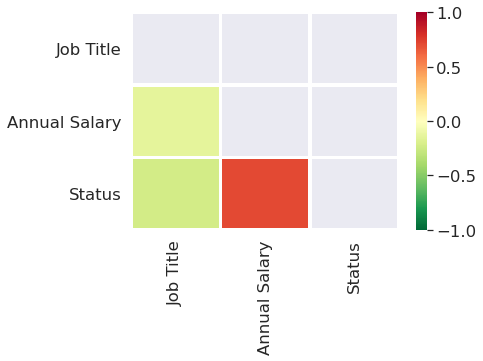
\includegraphics[width=0.475\textwidth]{figures/san_francisco_rankingfacts1.png}}
        \end{figure}
    \end{frame}
    
    
    \begin{frame}{Other Design Choices}
        \begin{itemize}
            \item \textbf{Part-time employees removal}: most of the tuples removed related to women (Chicago); excessive amount of tuples removed (San Francisco).
            \item \textbf{FAIR-DB: discretization using more bins}: less and different final dependencies detected (Chicago and San Francisco).
            \item \textbf{FAIR-DB: choice of different dependencies}: 85.6\% (Chicago) and 92.5\% (San Francisco) of the dataset `problematic'.
            \item \textbf{Grouping of job titles}: overturning of the outcomes for Ranking Facts (Chicago dataset unfair for males and fair for females, for each statistical measure).
            \item \textbf{Voluntary introduction of bias}: results from each tool oriented toward unfair Chicago dataset, in which women are discriminated against (retaining 50\%, 75\%, and 90\% of the \textit{Annual Salary} value of female employees).
        \end{itemize}
    \end{frame}

    
    \section{Section 1}
    % Section page.
    \begin{frame}[plain]{}
        \sectionpage
    \end{frame}
    
    
    \begin{frame}{Slide 1}
        \lipsum[1]
    \end{frame}
    
    
    \subsection{Subsection 1.1}
    \begin{frame}[plain]{}
        \subsectionpage
    \end{frame}
    \begin{frame}
        This frame has an empty title.
        \vfill
        \begin{itemize}
            \item item 1
            \begin{itemize}
                \item item 1.1
                \item item 1.2
            \end{itemize}
            \item item 2
            \item item 3
        \end{itemize}
    \end{frame}
    
    
    \subsection{Subsection 1.2}
    % Slide without numbering.
    \begin{frame}[nonumber]{Slide 1.2 without numbering}
        \lipsum[2]
    \end{frame}
    
    
    \section[Short]{Section 2}
    \begin{frame}{Slide 2}
        \begin{block}{Block}
            Text.
        \end{block}
        \pause
        \begin{alertblock}{Alert block}
            Alert \alert{text}.
        \end{alertblock}
        \pause
        \begin{exampleblock}{Example block}
            Example \textcolor{greenPolimi}{text}.
        \end{exampleblock}
    \end{frame}
\end{document}
